\renewcommand{\inputfile}{\version\ - edited 2008-06-26 stabOrder}
% $Author$ $Date$

%\section{Stability ordering of cycle expansions}
%\label{s-StabOrd}
% extracted from \Chapter{recycle}{30aug2006}{Cycle expansions}


\section{Stability ordering of cycle expansions}

For generic flows it is often not clear what
% Poincar\'{e} section should be used, and how it should be
partition of the {\statesp} generates the ``optimal''
symbolic dynamics.  Stability ordering
does not require understanding dynamics in such detail:
if you can find the cycles, you can use
stability ordered cycle expansions.
Stability truncation
% requires only that all cycles up to given
% stability cutoff be determined, without
% requiring detailed understanding of the topology of the
% flow and symbolic dynamics. It
is thus
%much
easier to implement for
a generic dynamical system than the
curvature expansions \rf{DasBuch} that rely on knowledge of the
topology of the flow. 
% \PC{refer here to the thesis section} %\refeq{curvbin}
% which rely on finite subshift approximations
% to a given flow.

Cycles can be detected numerically by
searching a long trajectory for near recurrences.
The long trajectory method for detecting cycles
\PC{refer here to the thesis section} %\refsect{s_long_time}
preferentially finds
the least unstable cycles, regardless of their topological length.
Another practical advantage of the method (in contrast to
Newton method searches)
is that it only finds
cycles in a given connected ergodic component of {\statesp},
ignoring  isolated cycles or other ergodic regions
elsewhere in the {\statesp}.

Stability ordering was introduced by
Dahlqvist and Russberg\rf{DR91}. The 
crucial observation is that
stability is multiplicative, so shadowing is approximately preserved
by including all terms with pseudocycle stability
\beq
\left|\ExpaEig_{p_1}\cdots\ExpaEig_{p_k}\right| \leq \stabCutoff
\ee{StabCutoff}
and ignoring all more unstable pseudocycles. For bound flows
all trajectories remain confined for
all times, implying the conservation of material flow:
\beq
	1/\zeta(0,0) = 1+\sumprime_\pseudos
		{ (-1)^k \over
		|\ExpaEig_{p_1}\cdots \ExpaEig_{p_k}|} = 0
	\label{prob-cons}
\eeq
which we will try to verify for \KSe.



\section{Stability ordering for KS cycles}
\label{s-StOrdKS}

In this section we attempt to numerically check the
flow conservation sum rule \refeq{prob-cons} for \KS\ equation with $L=22$
using a set of $~10,000$ periodic and $~10,000$ relative
periodic orbits  computed by Davidchack\rf{Davidchack_priv}.
In reduced space both \rpo s and pre-\po s are periodic so they should
enter in the same way in dynamical zeta function calculations\ES{Or do we have to
count some multiplicity due to $\Dn{1}$ differently? There is a copy of any rpo
due to $\Dn{1}$ but we also only consider $1/2$ of each periodic orbit, so I think
we are fine.}. the dynamical zeta function $1/\zeta(0,0)$ was evaluated
from \refeq{prob-cons} with stability cutoff $\stabCutoff$ as
in \refeq{StabCutoff}. After $\stabCutoff\simeq1200$
dynamical zeta function grows, indicating that we are missing some cycles.
To find them we will really have to understand the geometry of the flow.

%%%%%%%%%%%%%%%%%%%%%%%%%%%%%%%%%%%%%%%%%%%%%%%%%%%%%%%%%%%%%%%
\begin{figure}
    \vspace*{-5pt}
\begin{center}
	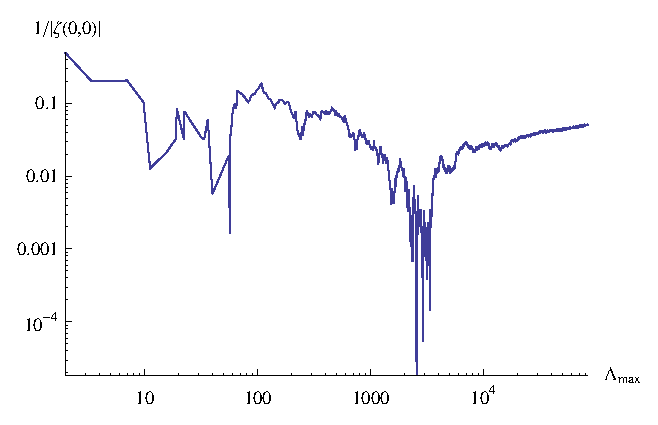
\includegraphics[width=0.75\textwidth]{../figs/ksStabOrder5000}
\end{center}
\caption[Flow conservation for \KS, $L=22$]
    {
Consistency check of flow conservation relation \refeq{prob-cons}
for \KS\ equation \refeq{ks} for $L=22$.
Here the dynamical zeta function $1/\zeta(0,0)$ was evaluated
from \refeq{prob-cons} with stability cutoff $\stabCutoff$ as
in \refeq{StabCutoff}. The maximum stability cutoff shown corresponds
to using the $5000$ least unstable cycles (\po s and \rpo s) in the set.
	}
\label{fig:zetaStabOrderKS22}
    \vspace*{-5pt}
\end{figure}
%%%%%%%%%%%%%%%%%%%%%%%%%%%%%%%%%%%%%%%%%%%%%%%%%%%%%%%%%%%%%%%%



